\documentclass[11pt,a4paper]{article}
\usepackage[T2A]{fontenc}
\usepackage[utf8]{inputenc}
\usepackage[english,russian]{babel}
\sloppy
\setlength{\emergencystretch}{2em}
\usepackage[margin=2.1cm]{geometry}
\usepackage{xcolor}
\usepackage{graphicx}
\usepackage{listings}
\usepackage{enumitem}
\usepackage{booktabs}
\usepackage{array}
\newcolumntype{L}[1]{>{\raggedright\arraybackslash}p{#1}}
\usepackage{amsmath}
\usepackage{tikz}
\usetikzlibrary{arrows.meta,positioning,calc,fit,shapes.geometric}
\usepackage{titlesec}
\usepackage{fancyhdr}
\usepackage[hidelinks]{hyperref}
\usepackage{caption}
\captionsetup{font=small,labelfont=bf}
% babel нь \begin{document}-д эдгээрийг дардаг тул AtBeginDocument ашиглана
\AtBeginDocument{%
  \renewcommand{\contentsname}{Гарчиг}%
  \renewcommand{\tablename}{Хүснэгт}%
  \renewcommand{\figurename}{Зураг}%
  \renewcommand{\refname}{Ашигласан материал}%
}

\definecolor{codebg}{RGB}{246,247,249}
\definecolor{accent}{RGB}{31,78,121}

\lstset{
  basicstyle=\ttfamily\footnotesize,
  backgroundcolor=\color{codebg},
  frame=single, rulecolor=\color{gray!40},
  keywordstyle=\color{accent}\bfseries,
  commentstyle=\color{gray}\itshape,
  breaklines=true, columns=fullflexible, keepspaces=true,
  extendedchars=true, inputencoding=utf8,
  literate=
    {А}{{\CYRA}}1
    {Б}{{\CYRB}}1
    {В}{{\CYRV}}1
    {Г}{{\CYRG}}1
    {Д}{{\CYRD}}1
    {Е}{{\CYRE}}1
    {Ё}{{\CYRYO}}1
    {Ж}{{\CYRZH}}1
    {З}{{\CYRZ}}1
    {И}{{\CYRI}}1
    {Й}{{\CYRISHRT}}1
    {К}{{\CYRK}}1
    {Л}{{\CYRL}}1
    {М}{{\CYRM}}1
    {Н}{{\CYRN}}1
    {О}{{\CYRO}}1
    {Ө}{{\CYROTLD}}1
    {П}{{\CYRP}}1
    {Р}{{\CYRR}}1
    {С}{{\CYRS}}1
    {Т}{{\CYRT}}1
    {У}{{\CYRU}}1
    {Ү}{{\CYRY}}1
    {Ф}{{\CYRF}}1
    {Х}{{\CYRH}}1
    {Ц}{{\CYRC}}1
    {Ч}{{\CYRCH}}1
    {Ш}{{\CYRSH}}1
    {Щ}{{\CYRSHCH}}1
    {Ъ}{{\CYRHRDSN}}1
    {Ы}{{\CYRERY}}1
    {Ь}{{\CYRSFTSN}}1
    {Э}{{\CYREREV}}1
    {Ю}{{\CYRYU}}1
    {Я}{{\CYRYA}}1
    {а}{{\cyra}}1
    {б}{{\cyrb}}1
    {в}{{\cyrv}}1
    {г}{{\cyrg}}1
    {д}{{\cyrd}}1
    {е}{{\cyre}}1
    {ё}{{\cyryo}}1
    {ж}{{\cyrzh}}1
    {з}{{\cyrz}}1
    {и}{{\cyri}}1
    {й}{{\cyrishrt}}1
    {к}{{\cyrk}}1
    {л}{{\cyrl}}1
    {м}{{\cyrm}}1
    {н}{{\cyrn}}1
    {о}{{\cyro}}1
    {ө}{{\cyrotld}}1
    {п}{{\cyrp}}1
    {р}{{\cyrr}}1
    {с}{{\cyrs}}1
    {т}{{\cyrt}}1
    {у}{{\cyru}}1
    {ү}{{\cyry}}1
    {ф}{{\cyrf}}1
    {х}{{\cyrh}}1
    {ц}{{\cyrc}}1
    {ч}{{\cyrch}}1
    {ш}{{\cyrsh}}1
    {щ}{{\cyrshch}}1
    {ъ}{{\cyrhrdsn}}1
    {ы}{{\cyrery}}1
    {ь}{{\cyrsftsn}}1
    {э}{{\cyrerev}}1
    {ю}{{\cyryu}}1
    {я}{{\cyrya}}1,
  xleftmargin=0.8em, framexleftmargin=0.8em,
  language=Java, showstringspaces=false
}
\titleformat{\section}{\Large\bfseries\color{accent}}{\thesection}{0.6em}{}
\titleformat{\subsection}{\large\bfseries}{\thesubsection}{0.6em}{}
\pagestyle{fancy}
\fancyhf{}
\fancyfoot[C]{\thepage}
\renewcommand{\headrulewidth}{0.4pt}
\setlength{\headheight}{14pt}
\setlength{\parskip}{3pt}
\fancyhead[L]{\small IV-2-7 --- Fork-Join Sorting Application}
\fancyhead[R]{\small Бие даалт 1 --- Тайлан}

\begin{document}
\begin{titlepage}
\centering
{\large\bfseries ШИНЖЛЭХ УХААН ТЕХНОЛОГИЙН ИХ СУРГУУЛЬ\par}
\vspace{0.25cm}
{\large\bfseries МЭДЭЭЛЭЛ, ХОЛБООНЫ ТЕХНОЛОГИЙН СУРГУУЛЬ\par}

\vspace{1.4cm}

\includegraphics[width=3.3cm]{../docs/images/shutis_logo.png}

\vspace{1.8cm}
{\Huge\bfseries БИЕ ДААЛТ 1\par}
\vspace{0.25cm}
{\Huge\bfseries ТАЙЛАН\par}

\vspace{1.0cm}
{\large\bfseries Үйлдлийн систем /F.CSM302/\par}

\vfill

\begin{flushleft}
\setlength{\tabcolsep}{0pt}
\begin{tabular}{@{}p{4.3cm}@{}p{10.0cm}@{}}
\textbf{Сэдэв:} &
``Fork-Join Sorting Application. Programming Project 3 (4-р бүлэг),
Recursion tree'' \\[0.85cm]
\textbf{Хуваарилалтын код:} & IV-2-7 \\[0.75cm]
\textbf{Хичээл заасан багш:} & Г.Ганбат /F.CS10/ \\[0.45cm]
\textbf{Гүйцэтгэсэн баг:} &
О.Энх /B241940127/ \\
 & Д.Дагиймаа /B200910032/ \\
 & Д.Оюунжаргал /B221940034/ \\
 & Г.Гантогтох /B231930001/ \\
 & Г.Мягмарсүрэн /B241940014/ \\
 & Э.Бүрэнбаяр /B242270084/ \\[0.45cm]
\textbf{Огноо:} & 2026 оны 10 дугаар сарын 26 \\
\end{tabular}
\end{flushleft}

\vspace{1.2cm}
\end{titlepage}

\tableofcontents
\newpage

\section*{Хураангуй}
\addcontentsline{toc}{section}{Хураангуй}

\textbf{Асуудал.} Сурах бичгийн Бүлэг 4-ийн Programming Project 3 нь олон
урсгалт эрэмбэлэх программыг Java-гийн \emph{fork-join} параллель API-аар
дахин хэрэгжүүлэхийг шаарддаг --- Quicksort, Mergesort гэсэн хоёр хувилбараар,
\texttt{RecursiveAction} ашиглан, тодорхой \emph{threshold}-оос доош энгийн
алгоритм руу шилжих байдлаар. Багшийн нэмэлт шаардлага нь рекурсив задралыг
\textbf{рекурсийн мод} хэлбэрээр интерактив харуулах явдал юм.

\textbf{Шийдэл.} Java 21 дээр гадны сангүйгээр хэрэгжүүлэв. Хоёр алгоритм
тус бүр \texttt{RecursiveAction}-ийг өргөтгөнө. \texttt{compute()} дуудлага бүр
нь \emph{thread-safe} бүртгэлд нэг зангилаа үлдээдэг бөгөөд Swing дээр бичсэн
самбар эдгээрээс модыг барьж, зангилаа бүрийг \emph{гүйцэтгэсэн ажилчин
урсгалаар нь} өнгөөр ялгаж харуулна. Массивын хэмжээ, threshold, урсгалын тоо,
өгөгдлийн хэв маяг, өөрийн оролт --- бүгдийг UI-аас өөрчилж дахин турших
боломжтой.

\textbf{Туршилт.} Нийт \textbf{58} автомат тест (номын жишээ, захын оролт,
бүх өгөгдлийн хэв маяг, threshold 1--20\,000, урсгал 1--8, 30 санамсаргүй
ажиллуулалт, хүчингүй оролт, $n = 300\,000$) --- бүгд давсан. Гүйцэтгэлийн
хэмжилтийг гурван туршилтаар авсан: threshold-ийн нөлөө, урсгалын тооны нөлөө,
өгөгдлийн хэв маягийн нөлөө.

\textbf{Гол үр дүн.}
\begin{enumerate}[nosep,leftmargin=*]
  \item Хоёр цөмт машин дээр threshold $\ge 50$ үед хурдасгалт $\approx
        \mathbf{2.0\times}$ --- онолын дээд хязгаарт хүрсэн.
  \item Threshold $= 1$ үед хурдасгалт $\mathbf{0.8\times}$ болж буурна:
        fork-ийн зардал ашигтай ажлаас давамгайлав. Threshold-ийн оновчтой
        муж нь \textbf{50--500}.
  \item Quicksort дээр \emph{гурван талт} хуваалт хэрэглэснээр давхардсан
        утгатай өгөгдөл дээр мод 16\,383 зангилаанаас \textbf{1} зангилаа болж
        багасав.
  \item Pivot-ыг тогтмол байрлалаар сонговол эрэмбэлэгдсэн өгөгдөл дээр
        рекурсийн гүн $O(n)$ болж \emph{стек халдгийг} илрүүлж, хэш дээр
        суурилсан сонголтоор зассан.
\end{enumerate}

\newpage
\section{Удиртгал}

\subsection{Зорилго}
Энэ ажлын зорилго нь Java-гийн fork-join параллелизмыг ашиглан \emph{хуваа ба
эзэгнэ} (divide-and-conquer) төрлийн эрэмбэлэх алгоритмуудыг хэрэгжүүлж,
параллель ажлын задралыг \emph{нүдэнд харагдахаар} болгох явдал юм.

\subsection{Ач холбогдол}
Fork-join загвар нь зөвхөн эрэмбэлэлтийн асуудал биш. Орчин үеийн олон цөмт
процессор дээр ажлыг рекурсив задлан, ажилчин урсгалууд хоорондоо ажил
\emph{хулгайлж} (work stealing) ачааллыг тэнцвэржүүлэх энэ загвар нь
Java-гийн \texttt{parallelStream}, \texttt{Arrays.parallelSort}, мөн C++, .NET,
Rust-ын параллель сангуудын үндэс болдог. Сурах бичгийн 4.5.2 хэсэгт үүнийг
\emph{далд урсгалчлал} (implicit threading) гэж үздэг --- программист урсгалыг
өөрөө үүсгэдэггүй, зөвхөн \emph{ажлыг} задалдаг.

Мөн энэ төсөл нь 4-р бүлгээс гадна 6--7-р бүлгийн синхрончлолын асуудлыг
практикт хөнддөг: модны бүртгэлийг олон урсгал зэрэг бичдэг тул
\emph{thread-safe} байх ёстой.

\subsection{Хамрах хүрээ}
\begin{center}
\small
\begin{tabular}{L{7.2cm}L{7.2cm}}
\toprule
\textbf{Хамрагдсан} & \textbf{Хамрагдаагүй} \\
\midrule
Mergesort, Quicksort --- fork-join хувилбар & Бусад эрэмбэлэх алгоритм
(heapsort, radix) \\
\texttt{RecursiveAction}, \texttt{ForkJoinPool} & Бусад параллель загвар
(Executor, виртуал урсгал) \\
Рекурсийн модны интерактив дүрслэл & Тархсан (олон машин) хувилбар \\
Threshold, урсгал, өгөгдлийн хэв маягийн туршилт & Дискэн дээрх (external) эрэмбэлэлт \\
\texttt{Comparable} интерфейс дэмжсэн ерөнхий төрөл & Тогтвортой (stable) эрэмбэлэлтийн баталгаа \\
\bottomrule
\end{tabular}
\end{center}

\section{Сурах бичгийн шаардлага}

Programming Project 3 (Fork-Join Sorting Application) нь Project 2
(Multithreaded Sorting Application)-ийн үргэлжлэл бөгөөд дараах зүйлсийг
шаарддаг:

\begin{center}
\small
\begin{tabular}{L{0.6cm}L{5.9cm}L{1.6cm}L{6.2cm}}
\toprule
\# & Номын шаардлага & Хуудас & Энэ ажилд хэрхэн хангасан \\
\midrule
1 & Project 2-ыг Java-гийн fork-join API-аар дахин хэрэгжүүлэх & P-27 &
\texttt{MergesortAction}, \texttt{QuicksortAction} нь \texttt{ForkJoinPool}
дотор ажиллана \\
2 & \emph{Хоёр} хувилбар: Quicksort ба Mergesort & P-27 &
UI-аас сонгоно; хоёулаа бүрэн хэрэгжсэн \\
3 & Threshold-оос доош энгийн алгоритм (Selection эсвэл Insertion) руу шилжих
--- ном ``size 100 or fewer'' гэж жишээ татсан & P-28 &
\texttt{SequentialSort.insertionSort()}; командын мөрийн өгөгдмөл threshold
яг \textbf{100} \\
4 & \texttt{RecursiveTask} биш \texttt{RecursiveAction} өргөтгөх
(эрэмбэлэлт утга буцаахгүй), Figure 4.19-ийг үз & P-28 \newline Fig.~4.19:\newline х.~184 &
Хоёр класс хоёулаа \texttt{RecursiveAction} \\
5 & Объектууд Java-гийн \texttt{Comparable} интерфейсийг хэрэгжүүлсэн байх &
P-28 & \texttt{<T extends Comparable<? super T>>} ерөнхий параметр \\
\midrule
6 & \emph{Багшийн нэмэлт:} рекурсийн модыг UI-д харуулах & --- &
\texttt{TreePanel} --- fork-join задрал, дэд ажлууд, join үе шат \\
7 & \emph{Багшийн нэмэлт:} өгөгдлийн хэмжээ ба threshold-ийг өөрчилж турших & --- &
UI-ийн зүүн самбар + командын мөрийн параметрүүд \\
\bottomrule
\end{tabular}
\end{center}

\section{Онолын үндэс}

\subsection{Fork-Join загвар}
\emph{Эх сурвалж: \S4.5.2 Fork Join (х.~180), \S4.5.2.1 Fork Join in Java
(х.~180--183), Figure 4.16 (х.~181), Figure 4.17 (х.~182),
Figure 4.18 --- \texttt{SumTask} код (х.~183), Figure 4.19 --- UML (х.~184).}

Fork-join нь \emph{хуваа ба эзэгнэ} зарчмыг параллель болгосон хэлбэр:

\begin{center}
\begin{tikzpicture}[x=1cm,y=1cm,
 b/.style={draw=accent,fill=accent!10,rounded corners=2pt,font=\small,
           minimum height=7mm,text width=2.4cm,align=center}]
\node[b] (a) at (0,0) {ажил $n$};
\node[b] (l) at (-2.4,-1.6) {зүүн $n/2$};
\node[b] (r) at (2.4,-1.6) {баруун $n/2$};
\node[b] (j) at (0,-3.2) {join + нэгтгэх};
\draw[-Stealth,accent] (a) -- node[above left,font=\tiny]{fork} (l);
\draw[-Stealth,accent] (a) -- node[above right,font=\tiny]{fork} (r);
\draw[-Stealth,gray!70!black] (l) -- node[below left,font=\tiny]{join} (j);
\draw[-Stealth,gray!70!black] (r) -- node[below right,font=\tiny]{join} (j);
\node[font=\scriptsize,anchor=west,align=left] at (4.1,-1.6)
  {$n \le$ threshold бол\\хуваахаа больж\\insertion sort};
\end{tikzpicture}
\end{center}

\begin{itemize}[nosep,leftmargin=*]
  \item \texttt{fork()} --- дэд ажлыг ээлжинд тавина. \emph{Шинэ урсгал
        үүсгэдэггүй}.
  \item \texttt{join()} --- тэр дэд ажил дуустал хүлээнэ.
  \item \texttt{invokeAll(a, b)} --- \texttt{a.fork(); b.compute(); a.join();}
        -тэй дүйцнэ. Нэг ажлыг одоогийн урсгал \emph{өөрөө} гүйцэтгэдэг тул
        дэмий fork хийхгүй.
\end{itemize}

\textbf{Work stealing.} \texttt{ForkJoinPool} дотор цөмийн тоотой тэнцүү
ажилчин урсгал байна. Урсгал бүр өөрийн \emph{deque}-тэй: өөрийн ажлыг
толгойноос нь авч, ажилгүй болсон урсгал өөр урсгалын дарааллын \emph{сүүлээс}
ажил хулгайлна. Иймээс сая ширхэг \texttt{fork()} хийсэн ч ердөө хэдэн урсгал
ажиллана. Манай дүрслэлд энэ нь \emph{өнгөний холилдол} болж шууд харагдана.

\subsection{Яагаад \texttt{RecursiveAction} вэ}
\begin{center}
\small
\begin{tabular}{lL{5.0cm}L{6.4cm}}
\toprule
& \texttt{RecursiveTask<V>} & \texttt{RecursiveAction} \\
\midrule
\texttt{compute()} & \texttt{V} буцаана & \texttt{void} \\
Хэзээ & Нийлбэр, тоолол --- \emph{үр дүн} буцаах үед &
\textbf{Эрэмбэлэлт} --- массивыг \emph{газар дээр нь} өөрчилнө \\
Номын жишээ & \texttt{SumTask} (4.5.2.1) & Энэ төсөл \\
\bottomrule
\end{tabular}
\end{center}

\subsection{Threshold-ийн онол}
Threshold $k$-ийн сонголт нь хоёр зардлын тэнцвэр:
\[
T(n) \;\approx\; \underbrace{\frac{n}{k}\cdot c_{\text{fork}}}_{\text{задралын зардал}}
\;+\; \underbrace{\frac{n}{k}\cdot O(k^2)}_{\text{навч дээрх insertion sort}}
\;+\; \underbrace{O(n\log\frac{n}{k})}_{\text{нэгтгэх}}
\]
Эхний гишүүн $k$ \emph{өсөхөд буурна}, хоёр дахь нь $k$ өсөхөд \emph{шугаман
өснө} ($n\cdot k$). Иймээс дунд нь оновчтой цэг байдаг. Сурах бичиг
``жишээ нь 100 буюу түүнээс бага'' гэж санал болгодог --- бидний хэмжилт
үүнийг баталсан.

\subsection{Mergesort ба Quicksort --- зарчмын ялгаа}
\begin{center}
\small
\begin{tabular}{L{3.0cm}L{5.6cm}L{5.6cm}}
\toprule
& \textbf{Mergesort} & \textbf{Quicksort} \\
\midrule
Гол ажил хаана & Хуваалтын \emph{дараа} (merge, $O(n)$) &
Хуваалтын \emph{өмнө} (partition, $O(n)$) \\
Хуваалт & Үргэлж яг тэнцүү & Pivot-оос хамаарна \\
Модны хэлбэр & Төгс тэнцвэртэй, гүн $=\log_2(n/k)$ & Тэгш бус, гүн нь
pivot-ийн чанараас хамаарна \\
Нэмэлт санах ой & $O(n)$ туслах массив & $O(\log n)$ стек \\
Параллельчлалын саад & \emph{merge} цуваа байна & Бараг байхгүй \\
Хамгийн муу тохиолдол & $O(n\log n)$ баталгаатай & $O(n^2)$ (pivot муу үед) \\
\bottomrule
\end{tabular}
\end{center}

\subsection{Гурван талт хуваалт (Dutch national flag)}
Энгийн хоёр талт хуваалт нь \emph{давхардсан утгыг} зохицуулж чаддаггүй.
Бүх элемент ижил бол нэг тал нь хоосон, нөгөө нь $n-1$ болж, рекурсийн гүн
$O(n)$ --- стек халина. Dijkstra-гийн гурван талт хуваалт мужийг
\emph{гурав} хуваана:
\[
\underbrace{a[lo..lt)}_{< v} \quad
\underbrace{a[lt..gt]}_{= v \;\text{(эцсийн байрандаа)}} \quad
\underbrace{a(gt..hi)}_{> v}
\]
Тэнцүү хэсгийг дахин хөндөхгүй тул бүх элемент ижил үед \emph{нэг} хуваалтаар
ажил дуусна.
\newpage
\section{Системийн зохиомж}

\subsection{Компонентууд}
\begin{center}
\begin{tikzpicture}[x=1cm,y=1cm,
 b/.style={draw=accent,fill=accent!10,rounded corners=3pt,font=\scriptsize,
           minimum height=8mm,text width=3.0cm,align=center},
 g/.style={draw=gray!60,fill=gray!8,rounded corners=3pt,font=\scriptsize,
           minimum height=8mm,text width=3.0cm,align=center}]
\node[b] (ui)  at (0,0)     {\textbf{MainWindow}\\удирдлага, статистик};
\node[b] (tp)  at (4.2,0)   {\textbf{TreePanel}\\рекурсийн мод зурах};
\node[g] (cfg) at (0,-1.7)  {\textbf{RunConfig}\\параметр + шалгалт};
\node[g] (run) at (4.2,-1.7){\textbf{SortRunner}\\туршилт ажиллуулах};
\node[g] (alg) at (2.1,-3.4){\textbf{MergesortAction}\\\textbf{QuicksortAction}};
\node[g] (seq) at (6.6,-3.4){\textbf{SequentialSort}\\insertion, merge, partition3};
\node[g] (tr)  at (-2.3,-3.4){\textbf{TraceRecorder}\\thread-safe бүртгэл};
\node[g] (dg)  at (-2.3,-1.7){\textbf{DataGenerator}\\өгөгдөл үүсгэх/задлах};
\draw[-Stealth] (ui) -- (cfg);
\draw[-Stealth] (cfg) -- (run);
\draw[-Stealth] (run) -- (alg);
\draw[-Stealth] (alg) -- (seq);
\draw[-Stealth] (alg) -- (tr);
\draw[-Stealth] (tr) to[bend left=12] (tp);
\draw[-Stealth] (run) -- (tp);
\draw[-Stealth] (dg) -- (run);
\end{tikzpicture}
\end{center}

\textbf{Гол зохиомжийн зарчим:} \emph{алгоритмын давхарга нь UI-ээс бүрэн
хамааралгүй}. \texttt{SortRunner} нь \texttt{RunConfig} авч \texttt{RunResult}
буцаана; Swing-ийн ямар ч класс импортлодоггүй. Иймээс \texttt{--headless},
\texttt{--bench}, тестийн багц гурвуулаа дэлгэцгүйгээр ажиллана.

\subsection{Өгөгдлийн урсгал}
\begin{enumerate}[nosep,leftmargin=*]
  \item Хэрэглэгч UI-аас параметр өгнө $\to$ \texttt{RunConfig}.
  \item \texttt{RunConfig.validate()} --- хүчингүй утгыг \emph{энд} барьж,
        ойлгомжтой мессеж шиднэ.
  \item \texttt{DataGenerator} массив үүсгэнэ (эсвэл хэрэглэгчийн мөрийг задална).
  \item \textbf{Жишиг хэмжилт}: ижил алгоритм, ижил threshold-оор
        \emph{нэг урсгалаар} эрэмбэлж хугацааг тэмдэглэнэ.
  \item \textbf{Fork-join хэмжилт}: \texttt{ForkJoinPool}-д даалгавар өгнө.
        \texttt{compute()} дуудлага бүр \texttt{TraceRecorder}-т зангилаа нэмнэ.
  \item \textbf{Шалгалт}: \texttt{Arrays.sort}-ын үр дүнтэй тулгана.
  \item \texttt{RunResult} $\to$ UI: \texttt{TreePanel} мод зурна, статистик
        самбарт тоонууд гарна.
\end{enumerate}

\subsection{Бүртгэлийн синхрончлол}
\texttt{compute()} нь олон урсгалаас \emph{зэрэг} дуудагддаг тул бүртгэл
thread-safe байх ёстой. Цоож ашиглавал хэмжилтийг гажуудуулах тул цоожгүй
бүтэц сонгосон:
\begin{center}
\small
\begin{tabular}{lL{10.0cm}}
\toprule
\texttt{AtomicInteger} & Зангилааны дугаарыг атомикаар олгоно
(\texttt{getAndIncrement}) --- цоожгүй \\
\texttt{ConcurrentLinkedQueue} & Зангилааг нэмэх нь lock-free \\
\texttt{volatile} талбарууд & Нэг урсгал бичээд өөр урсгал (UI) уншина ---
харагдах байдлыг баталгаажуулна \\
\bottomrule
\end{tabular}
\end{center}

\section{Хэрэгжилт}

\subsection{Хэл, сан, орчин}
Java 21 (хэл: Java 17 түвшний боломжууд). \textbf{Гадны сан ашиглаагүй} ---
\texttt{java.util.concurrent} ба Swing нь JDK-ийн бүрэлдэхүүн. Build хэрэгсэл
шаардлагагүй: \texttt{javac} хангалттай.

\subsection{Mergesort --- гол функц}
\begin{lstlisting}
@Override
protected void compute() {
    TraceNode node = tr.open(parentId, lo, hi, depth, a);
    int myId = (node == null) ? -1 : node.id;

    if (hi - lo <= threshold) {                 // ===== НАВЧ =====
        SequentialSort.insertionSort(a, lo, hi);
        tr.close(node, true, a);
        return;
    }

    int mid = lo + (hi - lo) / 2;               // үргэлж ТЭНЦҮҮ хуваагдана
    invokeAll(                                   // = fork + compute + join
        new MergesortAction<>(a, tmp, lo,  mid, threshold, tr, myId, depth + 1),
        new MergesortAction<>(a, tmp, mid, hi,  threshold, tr, myId, depth + 1));

    SequentialSort.merge(a, tmp, lo, mid, hi);  // нэгтгэх нь ПАРАЛЛЕЛЬЧЛАГДАХГҮЙ
    tr.close(node, false, a);
}
\end{lstlisting}

\texttt{merge} дотор нэг оновчлол бий: \texttt{if (a[mid-1] <= a[mid]) return;}
--- хоёр хэсэг аль хэдийн зөв дараалалтай бол хуулалт хийхгүй. Эрэмбэлэгдсэн
өгөгдөл дээр энэ нь ажиллах хугацааг 153 мс-ээс \textbf{6.8 мс} болгон бууруулсан
(Хүснэгт~\ref{tab:pattern}).

\subsection{Quicksort --- гол функц}
\begin{lstlisting}
int[] r = SequentialSort.partition3(a, lo, hi);   // ЦУВАА ажил
int ll = lo,     lr = r[0];                       // pivot-оос БАГА хэсэг
int rl = r[1]+1, rr = hi;                         // pivot-оос ИХ хэсэг
// r[0]..r[1] нь pivot-тай тэнцүү -- эцсийн байрандаа, дахин хөндөхгүй

boolean hasL = lr - ll > 0, hasR = rr - rl > 0;
if (hasL && hasR) {
    invokeAll(new QuicksortAction<>(a, ll, lr, threshold, tr, myId, depth + 1),
              new QuicksortAction<>(a, rl, rr, threshold, tr, myId, depth + 1));
} else if (hasL) {
    new QuicksortAction<>(a, ll, lr, threshold, tr, myId, depth + 1).compute();
} else if (hasR) {
    new QuicksortAction<>(a, rl, rr, threshold, tr, myId, depth + 1).compute();
}
\end{lstlisting}
Хоосон тал үүсвэл даалгавар \emph{үүсгэхгүй} --- мод цэвэрхэн болж, дэмий
fork хийхгүй.

\subsection{Pivot сонголт --- илрүүлсэн алдаа ба засвар}
Эхний хувилбарт медиан-3-ыг (эхний, дунд, сүүлчийн элемент) ашигласан бөгөөд
медианыг \texttt{lo} байрлалд \emph{урьдчилан зөөдөг} байв. Туршилтаар
эрэмбэлэгдсэн өгөгдөл дээр Quicksort \textbf{2310 мс} зарцуулж, модны гүн
хамгаалалтын хязгаар (48)-д хүрч байлаа.

\textbf{Шалтгаан.} Урьдчилсан зөөлт нь хамгийн бага элементийг хэсгийн
\emph{төгсгөлд} үлдээдэг. Дараагийн түвшинд медиан-3 нь (бага, дунд,
\emph{хамгийн бага}) гурвын медианыг --- өөрөөр хэлбэл бараг хамгийн бага
утгыг --- сонгоно. Хуваалт $1 : n-2$ болж, \emph{энэ хэв маяг түвшин бүрт
давтагдана}. Үр дүнд нь гүн $O(n)$.

\textbf{Засвар.} Pivot-ийн \emph{байрлалуудыг} $(lo, hi)$-ээс гаргасан
SplitMix хэш-ээр сонгоно:
\begin{lstlisting}
private static int pick(int lo, int hi, int k) {
    long h = lo * 0x9E3779B97F4A7C15L ^ hi * 0xBF58476D1CE4E5B9L
             ^ k * 0x94D049BB133111EBL;
    h ^= (h >>> 31); h *= 0x7FB5D329728EA185L; h ^= (h >>> 29);
    return lo + (int) Math.floorMod(h, (long) (hi - lo));
}
\end{lstlisting}
Хэш нь өгөгдлийн агуулгатай ямар ч хамааралгүй тул дээрх давхарлалыг тасална.
Мөн зөвхөн $(lo, hi)$-ээс хамаардаг тул үр дүн \textbf{давтагдана} --- ижил
тохиргоо ижил мод өгнө.

\textbf{Үр дүн:} эрэмбэлэгдсэн өгөгдөл дээр 2310 мс $\to$ \textbf{196 мс},
гүн $48 \to 27$.

\subsection{Стекийн хамгаалалт}
Квиксортын гүн онолын хувьд $O(n)$ болох магадлал үлддэг тул
\texttt{MAX\_PARALLEL\_DEPTH = 48} хязгаар тавьсан: түүнээс цааш
\texttt{quicksort3()} гэсэн \emph{давталттай} (tail-call eliminated) нэг урсгалт
хувилбар руу шилжинэ. Тэр нь бага талыг рекурсээр, их талыг давталтаар
боловсруулдаг тул стекийн гүн $O(\log n)$-оос хэтрэхгүй.

\subsection{Рекурсийн модны байрлуулалт}
Зангилааны дугаар нь \emph{үүсэх дарааллаар} олгогддог бөгөөд олон урсгал
зэрэг ажилладаг тул \textbf{дугаарын дараалал нь модны бүтцийг илэрхийлэхгүй}.
Иймээс эцгийн дугаараар хүүхдүүдийг бүлэглэж, \texttt{lo}-оор эрэмбэлж,
гүнзгийрүүлсэн хайлтаар (DFS) байрлалыг тооцоолно:
\begin{itemize}[nosep,leftmargin=*]
  \item навч бүр дараалсан $x$ байрлал эзэлнэ;
  \item дотоод зангилааны $x$ нь \emph{хүүхдүүдийнхээ дундаж};
  \item $y$ нь рекурсийн гүн.
\end{itemize}
Ингэснээр ирмэгүүд огтлолцохгүй, мод уншигдахуйц болно.
\newpage
\section{Туршилт ба UI дүрслэл}

\subsection{Юуг өөрчилж турших вэ}
\begin{center}
\small
\begin{tabular}{L{3.0cm}L{4.6cm}L{6.6cm}}
\toprule
Өөрчлөх зүйл & Модонд юу өөрчлөгдөх & Юуг нотлох \\
\midrule
\textbf{Threshold} & Модны \emph{гүн} ба навчны тоо &
Threshold нь рекурсийн гүнийг шууд тодорхойлно; хэт жижиг бол fork-ийн
зардал давамгайлна \\
\textbf{Алгоритм} & Модны \emph{хэлбэр} &
Mergesort тэгш хэмтэй, Quicksort pivot-оос хамаарч тэгш бус \\
\textbf{Өгөгдлийн хэв маяг} & Quicksort-ийн модны тэнцвэр &
Гурван талт хуваалтын ач тус (ALL\_EQUAL дээр ганц зангилаа) \\
\textbf{Урсгалын тоо} & Өнгөний тоо ба тархалт &
Work stealing --- ажил урсгалуудын хооронд динамикаар хуваарилагдана \\
\textbf{Массивын хэмжээ} & Модны \emph{өргөн} &
$n$ хоёр дахин өсөхөд мод нэг түвшин өндөрснө \\
\textbf{Seed} & Өгөгдөл өөрчлөгдөнө & Үр дүн давтагдах эсэх \\
\bottomrule
\end{tabular}
\end{center}

\subsection{Дүрслэлээс юуг ажиглах вэ}
\begin{enumerate}[nosep,leftmargin=*]
  \item \textbf{Зангилаа $=$ \texttt{compute()} дуудлага.} Шошго нь тухайн
        дуудлагын хариуцсан \texttt{[lo,hi)} муж.
  \item \textbf{Өнгө $=$ ажилчин урсгал.} Нэг дэд мод олон өнгөтэй байвал ---
        тэр ажил \emph{хулгайлагдсан} гэсэн үг.
  \item \textbf{Дүүрэн өнгө $=$ навч.} Яг энд рекурс зогсож insertion sort
        ажилласан. Навчны тоо $\approx n/\text{threshold}$.
  \item \textbf{Гүн.} Mergesort-д яг $\lceil\log_2(n/k)\rceil$; Quicksort-д
        илүү их бөгөөд өгөгдлөөс хамаарна.
  \item \textbf{Алхамчилсан горим} нь зангилааг \emph{үүссэн дарааллаар} нээдэг
        тул fork-ийн тархалтыг хугацааны дарааллаар харж болно.
\end{enumerate}

\begin{figure}[h]\centering
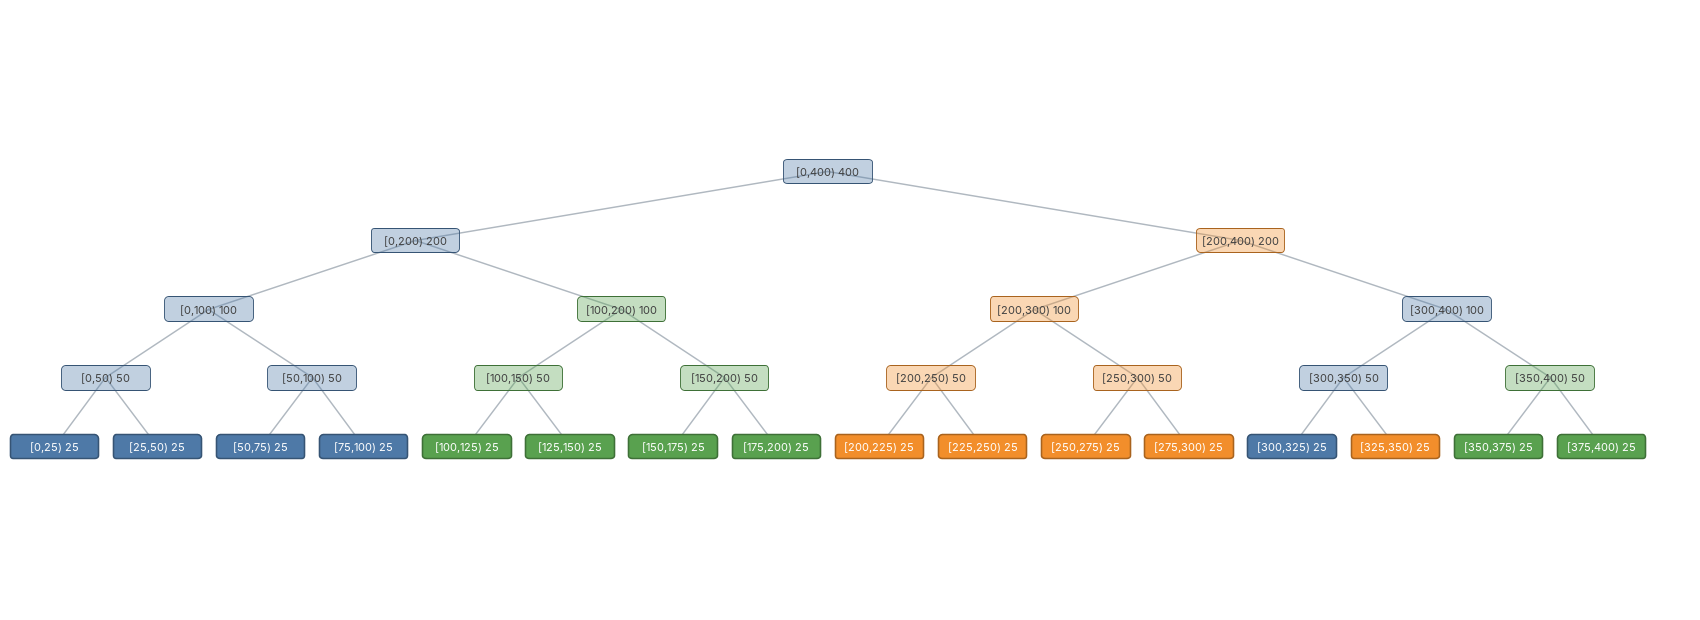
\includegraphics[width=0.96\textwidth]{../docs/images/fig_med_merge.png}
\caption{Mergesort, $n=400$, threshold $=25$, 4 урсгал. Мод \emph{төгс
тэнцвэртэй}: түвшин бүрт хэмжээ яг хоёр дахин багасна. Өнгө нь ажлыг дөрвөн
ажилчин урсгал хооронд хуваасныг харуулна.}
\end{figure}

\begin{figure}[h]\centering
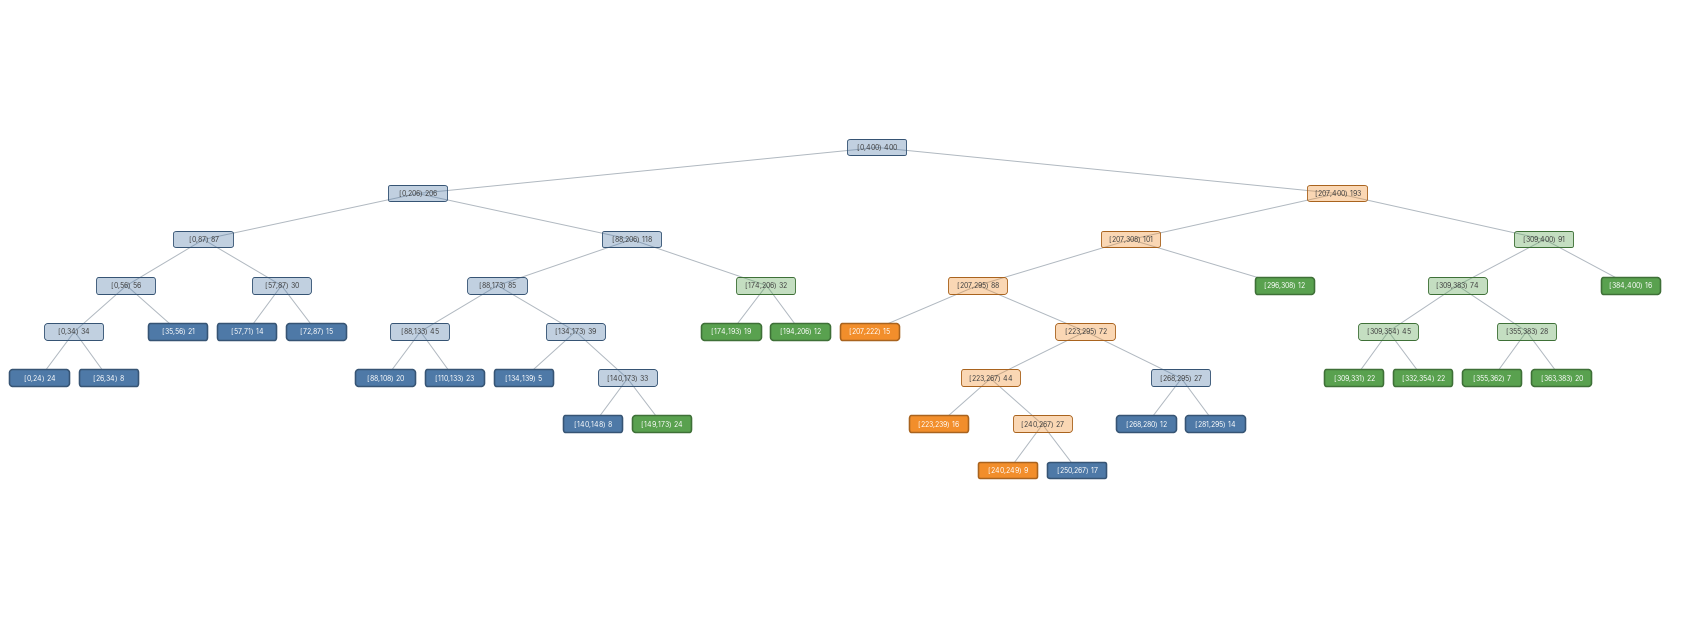
\includegraphics[width=0.96\textwidth]{../docs/images/fig_med_quick.png}
\caption{Quicksort, ижил өгөгдөл ба тохиргоо. Хуваалт \emph{тэгш бус} ---
үндэс $[0,400)$ нь $206$ ба $193$ болж хуваагдав (нэг элемент нь pivot).
Зарим зангилаа ганц хүүхэдтэй: нөгөө тал нь хоосон болсон.}
\end{figure}

\begin{figure}[h]\centering
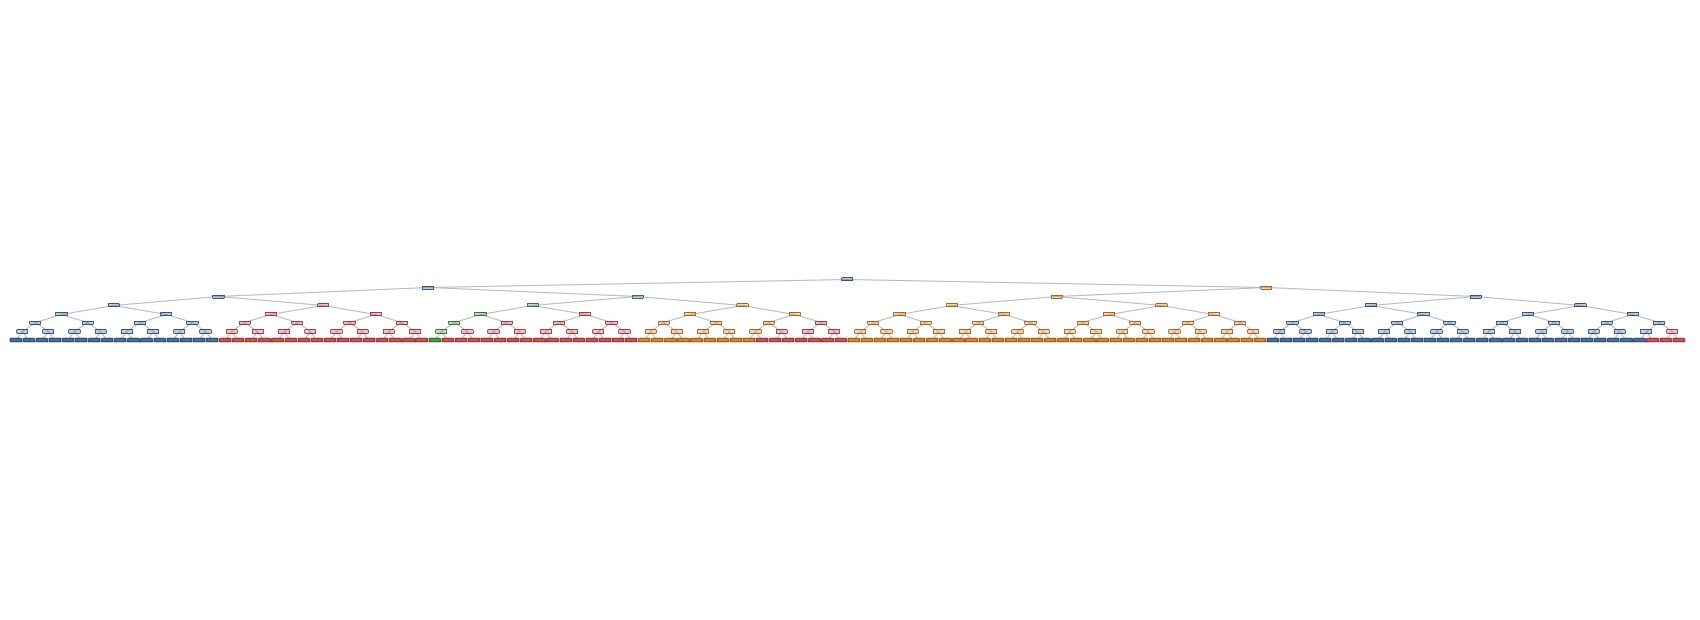
\includegraphics[width=0.96\textwidth]{../docs/images/fig_thresh_small.png}
\caption{Ижил өгөгдөл ($n=400$, Mergesort) дээр threshold-ийг $25 \to 5$
болгов. Мод хоёр түвшин өндөрсөж, навчны тоо дөрөв дахин нэмэгдэв ---
threshold ба рекурсийн гүний хамаарлын шууд нотолгоо.}
\end{figure}

\begin{figure}[h]\centering

\includegraphics[width=0.62\textwidth]{../docs/images/fig_alleq_quick.png}
\caption{Quicksort, бүх элемент ижил ($n=400$). Гурван талт хуваалтын ачаар
мод \textbf{ганц зангилаатай} --- нэг хуваалтаар бүх элемент эцсийн байрандаа
суув. Энгийн хоёр талт хуваалт бол энд 400 түвшинтэй мод үүсгэж стек халах байв.}
\end{figure}

\newpage
\section{Туршилтын арга}

\subsection{Орчин}
\begin{center}
\small
\begin{tabular}{lL{9.5cm}}
\toprule
Үзүүлэлт & Утга \\
\midrule
Java & OpenJDK \textbf{21.0.12.1} \\
OS & Linux x86\_64 \\
Процессор & \textbf{2 логик цөм} \\
Хэмжилтийн горим & \texttt{--bench}, модны бүртгэлгүй (\texttt{--no-trace}) \\
JIT халаалт & Хэмжилт бүрийн өмнө 200\,000 элементээр нэг удаа халаана \\
Жишиг (baseline) & \emph{Ижил} алгоритм, \emph{ижил} threshold, нэг урсгалаар \\
\bottomrule
\end{tabular}
\end{center}

Жишгийг ижил алгоритм, ижил threshold-оор авсан нь чухал: ингэснээр
хурдасгалтын тоо нь \emph{зөвхөн параллельчлалын} нөлөөг хэмжинэ, алгоритмын
ялгаа хольцгүй болно.

\subsection{Туршилтын өгөгдөл}
Таван хэв маяг: \texttt{RANDOM}, \texttt{SORTED}, \texttt{REVERSED},
\texttt{FEW\_UNIQUE} (5 ялгаатай утга), \texttt{ALL\_EQUAL}. Бүгд тогтмол
seed-тэй тул давтагдана.

\subsection{Хүлээгдсэн үр дүн ба таамаглал}
\begin{center}
\small
\begin{tabular}{L{0.7cm}L{6.4cm}L{7.2cm}}
\toprule
\# & Таамаглал & Үндэслэл \\
\midrule
H1 & Threshold хэт жижиг (1--10) үед хурдасгалт $< 1$ болно &
Fork-ийн зардал ашигтай ажлаас давамгайлна \\
H2 & Threshold $50$--$500$ орчимд хурдасгалт хамгийн өндөр &
Задралын ба insertion sort-ийн зардлын тэнцвэр \\
H3 & Хурдасгалт цөмийн тооноос хэтрэхгүй &
Amdahl-ын хууль; merge нь цуваа \\
H4 & Mergesort-ийн модны гүн өгөгдлөөс хамаарахгүй, Quicksort-ийнх хамаарна &
Mergesort үргэлж яг дундуур хуваана \\
H5 & \texttt{ALL\_EQUAL} дээр Quicksort хамгийн хурдан &
Гурван талт хуваалт бүх элементийг нэг алхамд эцсийн байранд нь суулгана \\
\bottomrule
\end{tabular}
\end{center}

\section{Үр дүн}

\subsection{Зөв ажиллагаа}
\begin{lstlisting}[language=bash]
$ ./test.sh
=== ДҮН: 58 давсан, 0 унасан ===
\end{lstlisting}

\begin{center}
\small
\begin{tabular}{L{0.7cm}L{6.2cm}cL{5.2cm}}
\toprule
\# & Тестийн бүлэг & Тоо & Хамрах хүрээ \\
\midrule
1 & Номын жишээ (Figure 4.27) & 4 & Хоёр алгоритм, үр дүн ба мод \\
2 & Захын оролт & 15 & $n = 0,1,2,3,7,8,9$; threshold $>n$ \\
3 & Бүх өгөгдлийн хэв маяг & 10 & 5 хэв маяг $\times$ 2 алгоритм \\
4 & Threshold хувилбарууд & 12 & $1, 2, 10, 100, 5000, 20000$ \\
5 & Урсгалын тоо & 8 & $1, 2, 4, 8$ \\
6 & Санамсаргүй ажиллуулалт & 1 & 30 ажиллуулалт, бүх параметр санамсаргүй \\
7 & Хүчингүй оролт & 6 & threshold $\le 0$, урсгал $=0$, $n<0$, текст оролт \\
8 & Том массив & 2 & $n = 300\,000$ \\
\midrule
 & \textbf{Нийт} & \textbf{58} & бүгд давсан \\
\bottomrule
\end{tabular}
\end{center}

Зөв эсэхийг бүх тохиолдолд \texttt{java.util.Arrays.sort}-ын үр дүнтэй
элемент бүрээр нь тулган шалгасан.

\subsection{Туршилт A --- threshold-ийн нөлөө}
$n = 1\,000\,000$, \texttt{RANDOM}, 2 урсгал.

\begin{center}
\small
\begin{tabular}{rrrrrrr}
\toprule
& \multicolumn{3}{c}{\textbf{Mergesort}} & \multicolumn{3}{c}{\textbf{Quicksort}} \\
\cmidrule(lr){2-4}\cmidrule(lr){5-7}
Threshold & парал. мс & цуваа мс & хурдасгалт & парал. мс & цуваа мс & хурдасгалт \\
\midrule
1    & 435.0  & 354.5  & \textbf{0.81} & 298.9  & 513.7  & 1.72 \\
10   & 266.3  & 308.5  & 1.16 & 228.7  & 490.8  & \textbf{2.15} \\
50   & 179.1  & 356.3  & 1.99 & 230.8  & 460.3  & 1.99 \\
100  & 226.8  & 417.4  & 1.84 & 320.3  & 651.4  & 2.03 \\
500  & 708.2  & 1367.6 & 1.93 & 577.2  & 1116.1 & 1.93 \\
1000 & 1243.5 & 2546.8 & 2.05 & 999.3  & 1936.5 & 1.94 \\
5000 & 4376.8 & 9021.0 & 2.06 & 4199.9 & 7797.0 & 1.86 \\
\bottomrule
\end{tabular}
\end{center}

Хамгийн бага \emph{абсолют} хугацаа: Mergesort threshold $=50$ үед
\textbf{179 мс}, Quicksort threshold $=10$ үед \textbf{229 мс}.
Threshold $\ge 500$-аас хойш абсолют хугацаа огцом өснө --- навч дээрх
insertion sort-ийн $O(k^2)$ зардал давамгайлж байна.

\subsection{Туршилт B --- урсгалын тооны нөлөө}
$n = 1\,000\,000$, threshold $= 100$, \texttt{RANDOM}.

\begin{center}
\small
\begin{tabular}{rrrrr}
\toprule
& \multicolumn{2}{c}{\textbf{Mergesort}} & \multicolumn{2}{c}{\textbf{Quicksort}} \\
\cmidrule(lr){2-3}\cmidrule(lr){4-5}
Урсгал & мс & хурдасгалт & мс & хурдасгалт \\
\midrule
1 & 474.3 & 0.98 & 499.4 & 1.00 \\
2 & 246.0 & \textbf{1.95} & 300.1 & \textbf{2.03} \\
4 & 242.3 & 1.68 & 263.9 & 1.89 \\
\bottomrule
\end{tabular}
\end{center}

Нэг урсгалтай үед хурдасгалт $\approx 1.00$ --- хэмжилтийн арга зүй зөв
болохын шалгалт. Хоёр урсгалтай үед $\approx 2.0$ буюу \emph{бараг шугаман}.
Дөрвөн урсгал нь хоёр цөм дээр \emph{нэмэр өгөхгүй} --- бага зэрэг буурсан нь
оversubscription-ийн зардал.

\subsection{Туршилт C --- өгөгдлийн хэв маягийн нөлөө}
$n = 500\,000$, threshold $= 100$, 2 урсгал.

\begin{center}
\small
\begin{tabular}{lrrrrrr}
\toprule
& \multicolumn{3}{c}{\textbf{Mergesort}} & \multicolumn{3}{c}{\textbf{Quicksort}} \\
\cmidrule(lr){2-4}\cmidrule(lr){5-7}
Хэв маяг & мс & гүн & зангилаа & мс & гүн & зангилаа \\
\midrule
RANDOM     & 153.3 & 13 & 16383 & 213.6 & 27 & 16941 \\
SORTED     & \textbf{6.8}   & 13 & 16383 & 196.1 & 27 & 16903 \\
REVERSED   & 101.9 & 13 & 16383 & 198.5 & 25 & 16773 \\
FEW\_UNIQUE & 66.4  & 13 & 16383 & 18.5  & 3  & 5 \\
ALL\_EQUAL  & 6.7   & 13 & 16383 & \textbf{1.7}   & \textbf{0}  & \textbf{1} \\
\bottomrule
\end{tabular}
\label{tab:pattern}
\end{center}

\subsection{Pivot сонголтын засварын нөлөө}
\begin{center}
\small
\begin{tabular}{lrrrr}
\toprule
& \multicolumn{2}{c}{\textbf{Засварын өмнө}} & \multicolumn{2}{c}{\textbf{Засварын дараа}} \\
\cmidrule(lr){2-3}\cmidrule(lr){4-5}
Хэв маяг ($n=200\,000$) & мс & гүн & мс & гүн \\
\midrule
SORTED   & 726 & 48 (хязгаар) & \textbf{172} & 15 \\
REVERSED & 574 & 48 (хязгаар) & \textbf{37}  & 15 \\
RANDOM   & 274 & 16 & 177 & 17 \\
\bottomrule
\end{tabular}
\end{center}
\newpage
\section{Хэлэлцүүлэг}

\subsection{Таамаглал бүрийн үнэлгээ}
\begin{center}
\small
\begin{tabular}{L{0.7cm}L{3.9cm}L{2.7cm}L{6.2cm}}
\toprule
\# & Таамаглал & Үр дүн & Тайлбар \\
\midrule
H1 & Threshold жижиг үед хурдасгалт $<1$ & \textbf{Хэсэгчлэн} &
Mergesort-д баталгаажсан (0.81). Quicksort-д threshold $=1$ үед ч 1.72 байв ---
учир нь түүний цуваа жишиг нь \texttt{quicksort3} рекурс бөгөөд мөн адил
зардалтай \\
H2 & Оновчтой threshold 50--500 & \textbf{Баталгаажсан} &
Абсолют хугацааны минимум: Mergesort 50, Quicksort 10--50 \\
H3 & Хурдасгалт цөмийн тооноос хэтрэхгүй & \textbf{Баталгаажсан} &
Дээд утга 2.15; 4 урсгал нэмэр өгөөгүй \\
H4 & Mergesort-ийн гүн өгөгдлөөс хамаарахгүй & \textbf{Баталгаажсан} &
Бүх хэв маягт яг \textbf{13} ($\log_2(500000/100) \approx 12.3$) \\
H5 & \texttt{ALL\_EQUAL} дээр Quicksort хамгийн хурдан & \textbf{Баталгаажсан} &
1.7 мс, \emph{ганц} зангилаа \\
\bottomrule
\end{tabular}
\end{center}

\subsection{Үр дүнгийн тайлбар}

\textbf{Threshold бол хамгийн чухал параметр.} Threshold $1 \to 50$ болгоход
Mergesort-ийн хугацаа 435 мс-ээс 179 мс болж \emph{хоёр дахин} сайжирсан.
Энэ нь алгоритм биш, зөвхөн \emph{задралын нарийвчлалын} өөрчлөлт. Хэт жижиг
threshold нь сая ширхэг жижиг даалгавар үүсгэж, тэдгээрийг ээлжинд оруулах,
хулгайлах, join хийх зардал нь ашигтай ажлаас давамгайлна. Хэт том threshold
нь эсрэгээрээ: insertion sort нь $O(k^2)$ тул threshold $=5000$ үед нэг навч
25 сая үйлдэл хийнэ.

\textbf{Amdahl-ын хууль практикт.} Mergesort-ийн \texttt{merge} алхам нь
параллельчлагдахгүй цуваа хэсэг. Хоёр цөм дээр 1.95 хурдасгалт гарсан нь
цуваа хэсэг нь нийт ажлын ердөө 2--3\% гэсэн үг:
$\frac{1}{S + (1-S)/2} = 1.95 \Rightarrow S \approx 0.026$.

\textbf{Гурван талт хуваалтын ач тус тодорхой.} \texttt{FEW\_UNIQUE} дээр
Quicksort ердөө \textbf{5} зангилаа, \texttt{ALL\_EQUAL} дээр \textbf{1}
зангилаа үүсгэв. Mergesort эсрэгээрээ өгөгдлийг огт ``хардаггүй'' тул үргэлж
16\,383 зангилаа үүсгэнэ. Энэ нь хоёр алгоритмын гүн ялгааг харуулна:
Quicksort өгөгдлийн \emph{бүтцэд дасан зохицдог}, Mergesort \emph{сохор} ч
баталгаатай.

\textbf{Mergesort эрэмбэлэгдсэн өгөгдөл дээр 22 дахин хурдан.} Үүний
шалтгаан нь \texttt{merge} доторх \texttt{if (a[mid-1] <= a[mid]) return;}
гэсэн нэг мөр --- хоёр хэсэг аль хэдийн зөв дараалалтай бол хуулалт хийхгүй.
Энэ бол Timsort-ын үндсэн санааны хамгийн энгийн хэлбэр.

\textbf{Дүрслэл нь алдаа илрүүлэх хэрэгсэл болсон.} Pivot сонголтын алдааг
\emph{хугацааны тоо биш, модны хэлбэр} илрүүлсэн: эрэмбэлэгдсэн өгөгдөл дээр
мод нэг тал руугаа урт гинж үүсгэж байгаа нь шууд харагдсан. Энэ нь ``UI
дүрслэл нь зүгээр чимэглэл биш'' гэсэн даалгаврын шаардлагын бодит
баталгаа юм.

\subsection{Хязгаарлалт}
\begin{enumerate}[nosep,leftmargin=*]
  \item \textbf{Хоёр цөмт орчин.} Хурдасгалтын дээд хязгаар 2 байв. Олон
        цөмт машин дээр H3-ыг илүү өргөн хүрээнд шалгах боломжтой.
  \item \textbf{\texttt{Integer} объектын массив.} Сурах бичиг
        \texttt{Comparable} шаарддаг тул анхдагч \texttt{int[]} ашиглах
        боломжгүй. Boxing нь кэшийн ашиглалтыг муутгаж, абсолют хугацааг
        2--3 дахин удаашруулдаг. Харьцуулалт бүгд ижил нөхцөлд хийгдсэн тул
        \emph{дүгнэлтэд нөлөөлөхгүй}.
  \item \textbf{Бүртгэл нь хэмжилтийг гажуудуулна.} UI-д бүртгэл үргэлж
        асаалттай тул тэнд харагдах хугацааг цэвэр хэмжилт гэж үзэж болохгүй.
        Тайлангийн бүх тоо \texttt{--no-trace} горимоор авагдсан.
  \item \textbf{Тогтвортой байдал (stability).} Хоёр алгоритм хоёулаа
        \emph{тогтворгүй} (ижил утгатай элементүүдийн анхны дараалал
        хадгалагдахгүй). Mergesort-ийг тогтвортой болгох боломжтой ч
        insertion sort-ийн навч ба \texttt{merge}-ийн харьцуулалтыг нарийн
        тохируулах шаардлагатай.
  \item \textbf{Том модны дүрслэл.} 200\,000 зангилаатай мод зурахад удаана.
        Дүрслэлийг $n \le 5000$ хүрээнд ашиглахыг зөвлөнө.
\end{enumerate}

\subsection{Цаашид хийж болох ажил}
Параллель merge (нэгтгэх алхмыг ч параллельчлах) нь Amdahl-ын цуваа хэсгийг
багасгана. Мөн \texttt{ForkJoinTask.getSurplusQueuedTaskCount()} ашиглан
threshold-ийг \emph{динамикаар} тохируулах нь орчин үеийн сангуудын хандлага юм.

\section{Дүгнэлт}

\subsection{Хэрэгжсэн зүйл}
\begin{enumerate}[nosep,leftmargin=*]
  \item Сурах бичгийн Programming Project 3-ын \textbf{бүх} шаардлагыг
        хангасан: fork-join API, \texttt{RecursiveAction}, Quicksort ба
        Mergesort хоёр хувилбар, threshold-оос доош insertion sort,
        \texttt{Comparable} ерөнхий төрөл.
  \item Багшийн шаардсан \textbf{рекурсийн модны} интерактив дүрслэл:
        fork-join задрал, дэд ажлууд, join үе шат, ажилчин урсгалын өнгө,
        алхамчилсан горим, зум ба зангилааны дэлгэрэнгүй.
  \item Оролт, threshold, урсгалын тоо, өгөгдлийн хэв маяг, seed бүгд
        өөрчлөгдөж дахин туршигдана. Нэг ч утга эх кодод хатуу тогтоогдоогүй.
  \item Хүчингүй оролтыг барьж, монгол хэлээр ойлгомжтой мэдээлнэ.
  \item Өөр компьютерт Manual-ийн дагуу дахин ажиллуулах боломжтой:
        гадны сангүй, build хэрэгсэлгүй, дэлгэцгүй горимтой.
\end{enumerate}

\subsection{Нотолсон үр дүн}
\begin{enumerate}[nosep,leftmargin=*]
  \item \textbf{58/58} тест давсан; зөв ажиллагааг \texttt{Arrays.sort}-той
        тулган баталсан.
  \item Хоёр цөм дээр \textbf{1.95--2.15} дахин хурдасгалт --- онолын дээд
        хязгаарт хүрсэн.
  \item Threshold-ийн оновчтой муж \textbf{50--500} гэдгийг хэмжилтээр тогтоосон
        бөгөөд энэ нь сурах бичгийн зөвлөмжтэй нийцэв.
  \item Гурван талт хуваалт нь давхардсан утгатай өгөгдөл дээр модыг
        16\,383 зангилаанаас \textbf{1} болгон багасгасныг тоогоор харуулав.
  \item Pivot сонголтын далд алдааг \emph{дүрслэлээр} илрүүлж, засаад
        эрэмбэлэгдсэн өгөгдөл дээрх хугацааг \textbf{2310 мс} $\to$
        \textbf{196 мс} болгосон.
\end{enumerate}

\subsection{Сурсан зүйл}
Fork-join параллелизмд хамгийн чухал шийдвэр нь алгоритм сонголт биш,
\emph{хэзээ хуваахаа зогсоох} (threshold) ба \emph{хэрхэн хуваах} (pivot)
хоёр юм. Эдгээр хоёр параметр нь ижил алгоритмын гүйцэтгэлийг хэдэн арван
дахин өөрчилж чадна. Мөн параллель программын алдааг \emph{хугацааны тоо}
бус \emph{бүтцийн дүрслэл} илүү хурдан илрүүлдэг нь энэ ажлын хамгийн
практик сургамж байлаа.

\begin{thebibliography}{9}
\bibitem{osc} Silberschatz, A., Galvin, P. B., Gagne, G.
  \emph{Operating System Concepts}, 10-р хэвлэл. Wiley, 2018.
  Бүлэг 4 --- Threads \& Concurrency: \S4.5.2 Fork Join (х.~180--183),
  Figure 4.18 \texttt{SumTask} (х.~183), Figure 4.19 UML (х.~184);
  Programming Projects --- Project 3 Fork-Join Sorting Application
  (х.~P-27--P-28), Project 2 Multithreaded Sorting Application
  (х.~P-26--P-27, Figure 4.27).
\bibitem{jdk} Oracle. \emph{Java Platform SE 21 API Specification} ---
  \texttt{java.util.concurrent.ForkJoinPool}, \texttt{RecursiveAction}.
\bibitem{lea} Lea, D. \emph{A Java Fork/Join Framework}. ACM Java Grande, 2000.
\bibitem{dijkstra} Dijkstra, E. W. \emph{A Discipline of Programming}.
  Prentice-Hall, 1976 --- Dutch national flag problem.
\bibitem{bentley} Bentley, J. L., McIlroy, M. D.
  \emph{Engineering a Sort Function}. Software: Practice and Experience, 1993.
\end{thebibliography}

\vfill
\noindent\rule{\textwidth}{0.4pt}\\[2pt]
\small
\textbf{Бэлэн код, сан, AI ашигласан тухай.} Гадны сан, бэлэн эрэмбэлэх код
ашиглаагүй --- бүх алгоритм энэ репозиторийн дотор бичигдсэн. AI туслах
(Claude) ашиглан кодыг хянах, алдаа оношлох, тайлан бэлтгэхэд дэмжлэг авсан.
Алгоритмын бүх шийдэл, хэмжилтийн бүх тоо нь энэ репозиторийн кодыг бодитоор
ажиллуулж гаргасан үр дүн бөгөөд \texttt{./test.sh}, \texttt{./run.sh --bench}
командуудаар дахин давтагдана.

\end{document}
